\documentclass{article}
\usepackage{tikz}
\usepackage{rotating}
\usetikzlibrary{arrows,shapes,positioning,shadows,trees}



\tikzset{
  basic/.style  = {draw, text width=2cm, drop shadow, font=\sffamily, rectangle},
  root/.style   = {basic, rounded corners=2pt, thin, align=center,
                   fill=green!30},
  level 2/.style = {basic, rounded corners=6pt, thin,align=center, fill=green!60,
                   text width=8em},
  level 3/.style = {basic, thin, align=left, fill=pink!60, text width=6.5em}
}

%To use line breaks you can use every tree node key and use center alignment.
\tikzset{every tree node/.style={align=center}}
%You can shorten the sibling distance to make it more compact.
\tikzset{sibling distance=6pt}
%You can also set the level distance
\tikzset{level distance=60pt}

\begin{document}
\begin{rotate}{90}

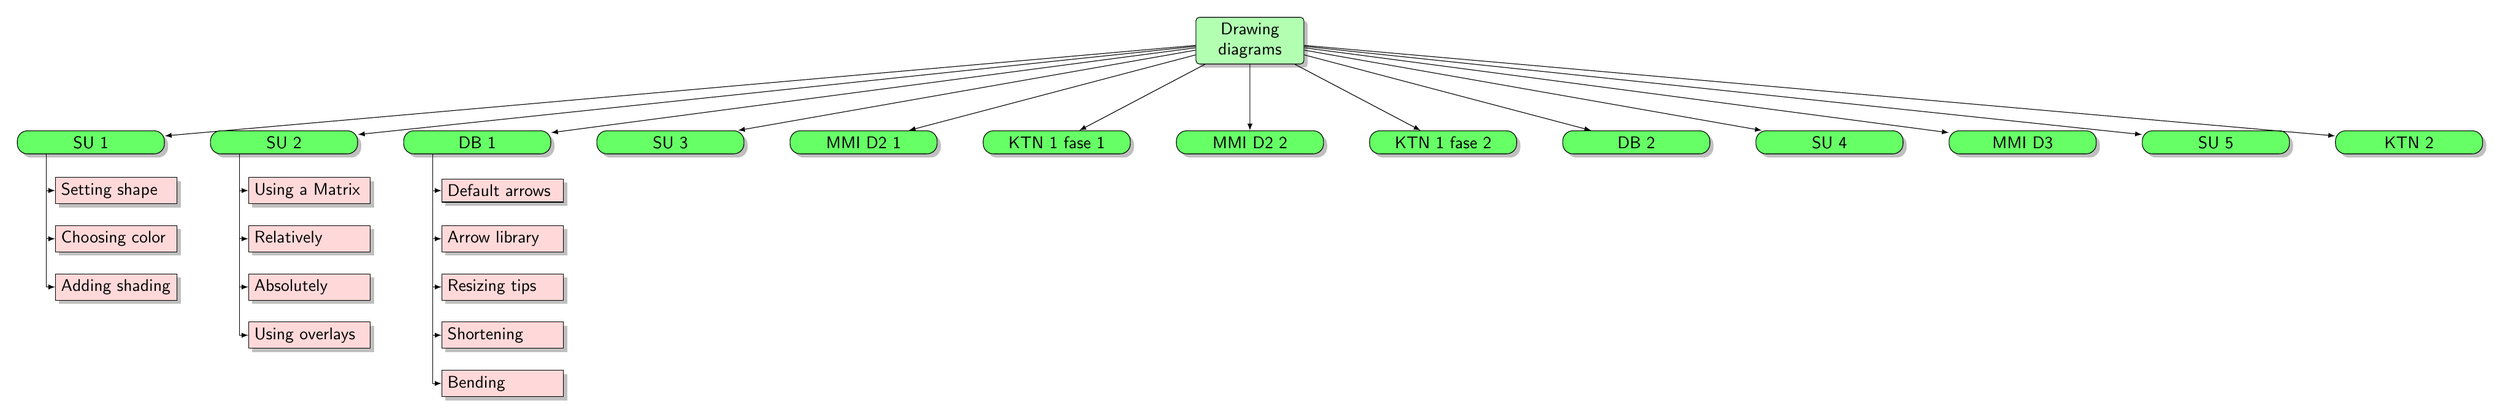
\begin{tikzpicture}[
  level 1/.style={sibling distance=40mm},
  edge from parent/.style={->,draw},
  >=latex]
  


% root of the the initial tree, level 1
\node[root] {Drawing diagrams}
% The first level, as children of the initial tree
child {node[level 2] (c1) {SU 1}}
child {node[level 2] (c2) {SU 2}}
child {node[level 2] (c3) {DB 1}}
child {node[level 2] (c4) {SU 3}}
child {node[level 2] (c5) {MMI D2 1}}
child {node[level 2] (c6) {KTN 1 fase 1}}
child {node[level 2] (c7) {MMI D2 2}}
child {node[level 2] (c8) {KTN 1 fase 2}}
child {node[level 2] (c9) {DB 2}}
child {node[level 2] (c10) {SU 4}}
child {node[level 2] (c11) {MMI D3}}
child {node[level 2] (c12) {SU 5}}
child {node[level 2] (c13) {KTN 2}};

% The second level, relatively positioned nodes
\begin{scope}[every node/.style={level 3}]
\node [below of = c1, xshift=15pt] (c11) {Setting shape};
\node [below of = c11] (c12) {Choosing color};
\node [below of = c12] (c13) {Adding shading};

\node [below of = c2, xshift=15pt] (c21) {Using a Matrix};
\node [below of = c21] (c22) {Relatively};
\node [below of = c22] (c23) {Absolutely};
\node [below of = c23] (c24) {Using overlays};

\node [below of = c3, xshift=15pt] (c31) {Default arrows};
\node [below of = c31] (c32) {Arrow library};
\node [below of = c32] (c33) {Resizing tips};
\node [below of = c33] (c34) {Shortening};
\node [below of = c34] (c35) {Bending};
\end{scope}

% lines from each level 1 node to every one of its "children"
\foreach \value in {1,2,3}
  \draw[->] (c1.195) |- (c1\value.west);

\foreach \value in {1,...,4}
  \draw[->] (c2.195) |- (c2\value.west);

\foreach \value in {1,...,5}
  \draw[->] (c3.195) |- (c3\value.west);
\end{tikzpicture}
\end{rotate}

\end{document}